% IMPORTANT! In order for the document to compile, one needs to use XeLaTeX or LuaLaTeX as compiler. This can be done in  Overleaf by Menu -> Settings -> Compiler -> Choose XeLaTeX/LuaLaTeX
\documentclass[t,24pt,serif,aspectratio=169]{beamer}

\setlength{\parskip}{\bigskipamount}

\usepackage{KUstyle}
\usepackage[style=authortitle,backend=biber]{biblatex}
\usepackage[]{float}
\usepackage{multicol} % Package for multiple coloumns
\usepackage{listings} % Package for code snippets
\usepackage{amsmath}
\usepackage{stmaryrd}

\newcommand{\cleftsemicirc}{\put(3.5,2.5){\oval(5,10)[l]}\put(3.5,-2.5){\line(0,0){10}}\phantom{\circ}}
\newcommand{\crightsemicirc}{\put(1.5,2.5){\oval(5,10)[r]}\put(1.5,-2.5){\line(0,0){10}}\phantom{\circ}}
\newcommand{\hole}{\cleftsemicirc \crightsemicirc}
\newcommand{\enc}[1]{\llbracket #1 \rrbracket}
\newcommand{\conf}[2]{\langle #1,#2 \rangle}

\lstset{basicstyle=\footnotesize\ttfamily,breaklines=true}
\lstset{frame=single}
\lstset{escapeinside={<@}{@>}}

\addbibresource{../report/references/ref.bib}


%\toplinje{Master's thesis} % The text at top. Remove the command if no text is desired

\begin{document}

% The first slide. One can for instance change the main title, the subtitle, speaker, KU-unit and date
{
\setbeamertemplate{background}{\includegraphics[width=\paperwidth,height=\paperheight]{KU/forside.pdf}}
\begin{frame}
    \begin{textblock*}{\textwidth}(0\textwidth,0.1\textheight)
        \begin{beamercolorbox}[wd=7.8cm,ht=7.3cm,sep=0.5cm]{hvidbox}
            \fontsize{5}{10}\fontfamily{ptm}\selectfont \textls[200]{UNIVERSITY OF COPENHAGEN}
            \noindent\textcolor{KUrod}{\rule{6.8cm}{0.4pt}}
        \end{beamercolorbox}
    \end{textblock*}
    \begin{textblock*}{\textwidth}(0\textwidth,0.1\textheight)
        \begin{beamercolorbox}[wd=7.8cm,sep=0.5cm]{hvidbox}
            \Large \textcolor{KUrod}{A Type Safe Calculus for Generating Syntax-Directed Editors}
            \vspace{0.5cm}
            \par
            \Large PEPM 2025
            \vspace{0.5cm}
            \par
            \normalsize \begin{verse}Benjamin Bennetzen \\
              Hans Hüttel \\
              Nikolaj Rossander Kristensen \\
              Sune Skaanning Engtorp \\
              Peter Buus Steffensen \end{verse}
        \end{beamercolorbox}
    \end{textblock*}
    \begin{textblock}{1}(6.3,11.38)
        \includegraphics[width=1cm]{KU/KU-logo.png}
    \end{textblock}
\end{frame}
}

\begin{frame}[hvid]
    \frametitle{Structure editors}

    Structure editors were introduced in order to avoid syntax errors.

    A structure editor builds the abstract syntax tree directly.
    
\end{frame}


\begin{frame}
    \frametitle{The Cornell Program Synthesizer}

    \begin{multicols}{2}
        Reps and Teitelbaum introduced the Cornell Program Synthesizer
        in 1981 for the PL/I language. In 1983 they presented the
        Synthesizer Generator, which can generate a structure for any
        programming language on the basis of a language definition. \footcite{timtom81}

       \vfill\null
       \columnbreak
        \includegraphics[width=0.4\textwidth]{img/cornell-ex.png}
    \end{multicols}
\end{frame}

\begin{frame}[hvid]
    \frametitle{Hazel and Hazelnut}

    \begin{multicols}{2}
        Omar et al.  (2019) developed the Hazel programming
        environment. With Hazel comes an editor calculus, which is a
        language for specifying edit operations. \footcite{omar}


        \columnbreak
        \includegraphics[width=0.5\textwidth]{img/hazel-ex.png}
    \end{multicols}
\end{frame}

\begin{frame}[hvid]
    \frametitle{Type-Safe Structure Editor Calculus}

    \begin{multicols}{2}
        \begin{itemize}
            \item<1-> The Type-Safe Structure Editor Calculus has been
                      developed in a series of student projects at UCPH and AAU \footcite{godiksen}

            \item<2-> The calculus was first implemented by a group of UCPH students\footcite{KU-bach}
            \footcite{aalborg}
        \end{itemize}

        \vfill\null\columnbreak
        \includegraphics<2->[width=0.5\textwidth]{img/ku-editor-ex.png}
    \end{multicols}
\end{frame}

\begin{frame}[hvid]
    \frametitle{Our work}
    \setbeamercovered{transparent}

    This talk presents a generalized version of the calculus and an
    encoding into a typed $\lambda$-calculus.

        \bigskip

    This has two significant advantages:
    
    \begin{itemize}
\item The encoding satisfies \alert{a general property of type-safety}:
    Well-typed editor scripts will always produce syntactically
    well-formed programs.
    
  \item It becomes possible to devise an editor generator in a typed
    functional programming language.
    \end{itemize}
    
\end{frame}

\begin{frame}
  \frametitle{Our work}

  \begin{itemize}
  \item An encoding and the proof of its soundness
    
  \item An implementation in Elm of an editor generator based on the
    encoding. Our criteria for a good implementation are:
              \begin{itemize}
                  \pause
                  \item Editing the abstract syntax of any program directly
                        \pause
                  \item Generic editing
                        \pause
                  \item Handling context-sensitive syntax
                        \pause
                  \item Multiple views of code being edited
                        \pause
                  \item A non-challenging way of specifying syntax
              \end{itemize}
            \end{itemize}

            We demonstrate the generality of our approach by showing
            how to handle three different language specifications.
    \setbeamercovered{invisible}
\end{frame}


\begin{frame}
  \frametitle{Abstract Syntax Trees}

  We use the presentation by Harper\footcite{harper} where an abstract
  syntax is defined by
  
    \begin{multicols}{2}
        \begin{itemize}
            \item A collection of sorts $\mathcal{S}$
            \item An arity-indexed family of operators $\mathcal{O}$
            \item A sort-indexed family of variables $\mathcal{X}$
        \end{itemize}

        \columnbreak
        \pause
        \begin{itemize}
            \item $\mathcal{S} = \{ exp \}$
            \item $plus \in \mathcal{O}_\alpha$ with arity $\alpha = (exp_1,exp_2)exp$
        \end{itemize}

    \end{multicols}

\end{frame}

\begin{frame}
  \frametitle{Abstract Binding Trees}

  Often a syntax will include binders. Following Harper, we can
  represent a syntax with binders as follows.
  
    \begin{multicols}{2}
        \begin{itemize}
            \item ASTs are enriched with bindings
            \item All operators are assigned generalized arity $(\vec{x_1}.x_1,...,\vec{x_n}.x_n)s$
        \end{itemize}
        \columnbreak
        \pause
        \begin{itemize}
            \item $\mathcal{S} = \{ exp, stmt \}$
            \item $let \in \mathcal{O}_\alpha$ with arity $\alpha = (exp_1,exp_2.stmt)stmt$
        \end{itemize}
    \end{multicols}

\end{frame}

\begin{frame}
  \frametitle{Generalized editor calculus}

  We now present an editor calculus for an arbitrary abstract syntax.
  
    \begin{itemize}
        \item Assume that the abstract syntax of a language is given by:
              \begin{enumerate}
                  \item A set of sorts $\mathcal{S}$
                  \item An arity-indexed family of operators $\mathcal{O}$
                  \item A sort-indexed family of variables $\mathcal{X}$
              \end{enumerate}
        \item Then, for every sort $s \in \mathcal{S}$, we add the following operators to $\mathcal{O}$
              \begin{enumerate}
                  \item A $hole_s$ operator with arity $()s$
                  \item A $cursor_s$ operator with arity $(s)s$
              \end{enumerate}
    \end{itemize}
\end{frame}

\begin{frame}
  \frametitle{Editor calculus}

  Our generalized editor calculus is defined by the formation rules
    \[
        \begin{aligned}
            E    & ::= \quad \underbrace{\pi.E}_{\text{prefixing}} \mid \underbrace{\phi \Rightarrow E_1|E_2}_{\text{conditional}} \mid
            \underbrace{E_1 \ggg E_2}_{\text{sequence}} \mid rec \ x.E \mid x \mid nil      &  &
            \text{\alert{edit actions}}\\
            \pi  & ::= \quad \underbrace{\textsf{child}\; n}_{\text{move down}} 
            \mid \underbrace{\textsf{parent}}_{\text{move up}} \mid
            \underbrace{\{ o \}}_{\text{insert operator}}                                                          &  & \text{\alert{prefixes}}\\
            \phi & ::= \quad \neg \phi \mid\phi \land \phi \mid\phi
            \lor \phi \mid @o \mid \Diamond o \mid\square o && \text{\alert{conditions}}
        \end{aligned}
      \]

Unlike the Hazel editor calculus this allows us to define
repetition-based editor scripts (using recursion).

The conditions allow us to make edit actions conditional on the shape
of the abstract syntax tree.

\end{frame}

\begin{frame}
    \frametitle{Cursorless trees}

    We first define trees without cursors. These are crucial for
    defining cursor contexts and well-formed trees. 

    \begin{enumerate}
        \item The sorts $\hat{\mathcal{S}} = \{ \hat{s} \}_{s \in \mathcal{S}}$
        \item The family of cursorless operators $\hat{\mathcal{O}}$ is made by adding
              the operator $\hat{o}$ of arity
              $(\vec{\hat{s}}_1.\hat{s}_1,...,\vec{\hat{s}}_n.\hat{s}_n)\hat{s}$
              for every $o \in \mathcal{O}$ of arity $(\vec{s}_1.s_1,...,\vec{s}_n.s_n)s$, excluding cursors
        \item The family of variables $\hat{\mathcal{X}}$
    \end{enumerate}
\end{frame}

\begin{frame}
    \frametitle{Cursor context}

    A cursor context holds information about the current tree
    surrounding the subtree where editing takes place.

    The cursor is just one more operator! We represent the cursor
    using an additional sort $C$ and an additional operator.
    
    \begin{enumerate}
        \item The sorts $\mathcal{S}^C = \hat{\mathcal{S}} \cup \{C\}$
        \item The family of operators $\mathcal{O}^C = \hat{\mathcal{O}}$ extended with the $[\cdot]$ operator with arity $()C$
        \item For every operator $\hat{o} \in \hat{\mathcal{O}}$ of
          arity
          $(\vec{\hat{s}}_1.\hat{s}_1,...,\vec{\hat{s}}_n.\hat{s}_n)\hat{s}$
          and for every $1 \leq i \leq n$ we introduce an operator $o_i^C$ of arity $(\vec{\hat{s}}_1.\hat{s}_1,...,\vec{\hat{s}}_i.C,...,\vec{\hat{s}}_n.\hat{s}_n)C$ to $\mathcal{O}^C$
        \item We have an extended family of variables $\mathcal{X}^C = \hat{\mathcal{X}}$
    \end{enumerate}
\end{frame}

\begin{frame}
    \frametitle{Well-formed trees}

    Trees should only contain a single cursor. If they do, we say that
    they are \alert{well-formed}.

    We can define the set of well-formed trees by
    
    \begin{enumerate}
        \item The sorts $\dot{\mathcal{S}} = \hat{\mathcal{S}} \cup \{ \dot{s} \}_{s \in \mathcal{S}}$
        \item The family of operators $\dot{\mathcal{O}} = \hat{\mathcal{O}}$ extended with an operator of arity $(\hat{s})\dot{s}$ for every $\hat{s} \in \hat{\mathcal{S}}$
        \item For every operator $\hat{o} \in \hat{\mathcal{O}}$ of arity $(\vec{\hat{s}}_1.\hat{s}_1,...,\vec{\hat{s}}_n.\hat{s}_n)\hat{s}$ and for every $1 \leq i \leq n$ the operator $\dot{o}_i$ of arity $(\vec{\hat{s}}_1.\hat{s}_1,...,\vec{\hat{s}}_i.\hat{s}_i,...,\vec{\hat{s}}_n.\hat{s}_n)\dot{s}$ is added to $\dot{\mathcal{O}}$
        \item The family of variables $\dot{\mathcal{X}} = \hat{\mathcal{X}}$
    \end{enumerate}
\end{frame}

\begin{frame}
    \frametitle{Semantics (Editor Expressions)}

    \[
        \text{(Cond-1)} \ \frac{a \models \phi}{\langle \phi \Rightarrow E_1|E_2, C[a] \rangle \stackrel{\epsilon}{\Rightarrow} \langle E_1, C[a] \rangle}
    \]

    \[
        \text{(Cond-2)} \ \frac{a \not\models \phi}{\langle \phi \Rightarrow E_1|E_2, C[a] \rangle \stackrel{\epsilon}{\Rightarrow} \langle E_2, C[a] \rangle}
    \]
    \[
        \text{(Context)} \ \frac{a \stackrel{\pi}{\Rightarrow} a'}{\langle \pi.E,C[a] \rangle \stackrel{\pi}{\Rightarrow} \langle E,C[a'] \rangle}
    \]
\end{frame}

\begin{frame}
    \frametitle{Semantics (Substitution and cursor movement)}
    \[
        \text{(Insert-op)} \ \frac{}{[\hat{a}] \stackrel{\{ o \}}{\Rightarrow} [o(\vec{x}_1.\hole_{s_1};...;\vec{x}_n.\hole_{s_n})]} \hat{a} \in \mathcal{B}[\mathcal{X}]_s \text{where } s \text{ is the sort of } o
    \]

    \vspace{1cm}

    \[
        \text{(Child-i)} \ \frac{}{[\hat{o}(\vec{x}_1.\hat{a}_1;...;\vec{x}_n.\hat{a}_n)] \stackrel{child \ i}{\Rightarrow} o(\vec{x}_1.\hat{a}_1;...;\vec{x}_i.[\hat{a}_i];...;\vec{x}_n.\hat{a}_n)}
    \]

    \[
        \text{(Parent)} \ \frac{}{o(\vec{x}_1.\hat{a}_1;...;\vec{x}_i.[\hat{a}_i];...;\vec{x}_n.\hat{a}_n) \stackrel{parent}{\Rightarrow} [\hat{o}(\vec{x}_1.\hat{a}_1;...;\vec{x}_n.\hat{a}_n)]}
    \]
\end{frame}

\begin{frame}
    \frametitle{Semantics (Conditionals)}
    \[
        \text{(Negation)} \ \frac{[\hat{a}] \not\models \phi}{[\hat{a}] \models \neg \phi}
    \]

    \[
        \text{(Conjunction)} \ \frac{[\hat{a}] \models \phi_1 \quad [\hat{a}] \models \phi_2}{[\hat{a}] \models \phi_1 \land \phi_2}
    \]

\end{frame}

\begin{frame}
    \frametitle{Semantics (Modal logic)}

    \[
        \text{(At-op)} \ \frac{}{[o(\vec{x}_1.\hat{a}_1;...;\vec{x}_n.\hat{a}_n)] \models @o}
    \]

    \[
        \text{(Possibly-i)} \ \frac{[\hat{a}_i] \models \Diamond o}{[o(\vec{x}_1.\hat{a}_1;...;\Vec{x}_i.\hat{a}_i;...;\vec{x}_n.\hat{a}_n)] \models \Diamond o}
    \]

    \[
        \text{(Possibly-trivial)} \ \frac{[\hat{a}] \models @o}{[\hat{a}] \models \Diamond o}
    \]

\end{frame}




\begin{frame}[hvid]
    \frametitle{Encoding the generalized editor calculus in an extended $\lambda$-calculus}
    \begin{itemize}
        \item Simply-typed $\lambda$-calculus with pairs, pattern matching and recursion
        \item Assuming that:
              \begin{itemize}
                  \item Type system of the simply-typed $\lambda$-calculus is sound
                  \item Encoding is correct
                  \item Then any instance of the editor will have a sound type system
              \end{itemize}
    \end{itemize}
\end{frame}

\begin{frame}[hvid]
    \frametitle{Extended $\lambda$-calculus}
    \begin{multicols}{2}
        \begin{center}
            Terms
            \[
                \begin{aligned}
                    M \quad   & ::= \lambda x : \tau.M                           & (abstraction)             &  & \\
                              & \quad | \quad M_1 M_2                            & (application)             &  & \\
                              & \quad | \quad x                                  & (variable)                &  & \\
                              & \quad | \quad o                                  & (operator)                &  & \\
                              & \quad | \quad (M_1,M_2)                          & \text{(pair)}             &  & \\
                              & \quad | \quad M.1                                & \text{(first projection)} &  & \\
                    ...                                                                                           \\
                    M,N \quad & ::= match \ M \ \overrightarrow{p \rightarrow N} & \text{(match construct)}  &  & \\
                    p \quad   & ::= x                                            & \text{(variable)}         &  & \\
                    ...       &                                                  &                           &  &
                \end{aligned}
            \]
        \end{center}
        \columnbreak
        \begin{center}
            Types
        \end{center}
        \[
            \begin{aligned}
                \tau \quad & ::= \tau_1 \rightarrow \tau_2      & (function)            &  & \\
                           & \quad | \quad s                    & (sort)                &  & \\
                           & \quad | \quad \tau_1 \times \tau_2 & \text{(product type)} &  & \\
                           & \quad | \quad Bool                 & \text{(boolean)}
            \end{aligned}
        \]

    \end{multicols}
\end{frame}

\begin{frame}[hvid]
    \frametitle{Encoding abts and editor expressions}
    \begin{itemize}
        \item Typing rules for operators
              \[
                  (\text{T-Operator}) \ \frac{o \in \mathcal{O} \text{ and has arity } (\Vec{s}_1.s_1,...,\Vec{s}_n.s_n)s}{\Gamma \vdash o : (\Vec{s}_1 \rightarrow s_1) \rightarrow ... (\Vec{s}_n \rightarrow s_n) \rightarrow s}
              \]
        \item Encoding of abts
              \[
                  \llbracket o(\Vec{x}_1.a_1,...,\Vec{x}_n.a_n) \rrbracket = o(\lambda \Vec{x}_1:\Vec{s}_1.\llbracket a_1 \rrbracket)...(\lambda \Vec{x}_n : \Vec{s}_n.\llbracket a_n \rrbracket)
              \]
        \item Encoding of editor expressions
              \begin{center}
                  \[
                      \llbracket \pi.E \rrbracket = \lambda CC : Ctx.\llbracket E \rrbracket ((\llbracket \pi \rrbracket C.1), C.2)
                  \]
                  ...
                  \[
                      \enc{\conf{E}{C[a']}} = \enc{E} \ (\enc{a}, \enc{C})
                  \]
              \end{center}
    \end{itemize}
\end{frame}




\begin{frame}[hvid]
  \frametitle{Implementation}

  In our implementation the important choices concern
  
    \begin{itemize}
        \item Representing syntax
        \item Code generation vs. generic model
        \item Generating source code
        \item Editor expressions
    \end{itemize}
\end{frame}


\begin{frame}
  \frametitle{Representing syntax}

  Early work on syntax specifications for structure editors includes
  
    \begin{itemize}
        \item Metal\footcite{metal}
              \pause
        \item Zephyr ASDL\footcite{zephyr}
              \pause
        \item ASN.1\footcite{asn1}
              \pause
            \end{itemize}

            The common problem: no support for binders.

\end{frame}

\begin{frame}
    \frametitle{Representing syntax (Continued)}
    \begin{multicols}{2}
       We have created our own specification language. Here is an
       example specification of a subset of SQL.
                  \vspace{1cm}

                  \includegraphics<2->[width=0.45\textwidth]{img/spec-lang-parseable-ex.png}

        \columnbreak
        \includegraphics[width=0.5\textwidth]{img/spec-lang-ex.png}
    \end{multicols}

\end{frame}

\begin{frame}[hvid]
  \frametitle{Generic model or code generation?}

  Should one use a generic model for the generalized editor or should
  one generate code for an editor instance?
  
    \begin{itemize}
        \item Generic model:
              \begin{itemize}
                  \item No need for code generation (less work and error prone)
                  \item However, this is less efficient and needs
                    thorough well-formedness checks 
              \end{itemize}
        \item Code generation:
              \begin{itemize}
                  \item Take advantage of algebraic data types (only well-formed terms can be created)
                  \item However, this requires code generation
              \end{itemize}
            \end{itemize}

            (Notice the similarity with the question of specialization
            in the work on partial evaluation.)
\end{frame}

\begin{frame}[hvid]
    \frametitle{Generating source code}
    \begin{multicols}{2}
        \begin{itemize}
            \item Elm CodeGen package\footfullcite{elm-codegen-package}
            \item Can be useful if integrated with language specification parser
        \end{itemize}
        \columnbreak
        \includegraphics[width=0.4\textwidth]{img/codegen-ex.png}
    \end{multicols}
\end{frame}

\begin{frame}[hvid]
    \frametitle{Generating source code (Continued)}
    \begin{center}
        \includegraphics[width=0.5\textwidth]{img/codegen-ex2.png}
    \end{center}
\end{frame}

\begin{frame}[hvid]
    \frametitle{Generating Editor Expression Code}
       How do we decompose an AST into a cursor context and well-formed tree? 
       
       \bigskip

       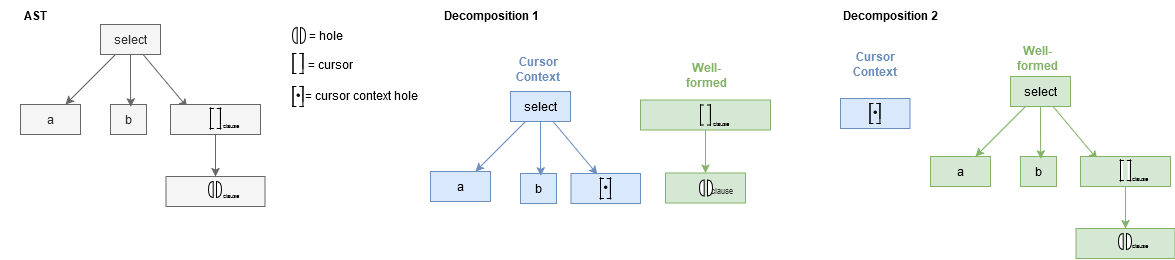
\includegraphics[width=1\textwidth]{img/slq-decompose-ex-wide.drawio.png}
\end{frame}


\begin{frame}[hvid]
    \frametitle{Generating Editor Expression Code}
       We must be able to do this in exactly one way. The
       algorithm for unique decomposition will
                  \begin{itemize}
                      \item Generate a path to the cursor
                      \item Generate an abt of sort $s^C \in \mathcal{S}^C$ based on the path and stop at the cursor
                      \item Generate an abt of sort $\dot{s} \in \dot{\mathcal{S}}$
                            based on the rest of the tree that was not traversed
                  \end{itemize}
\end{frame}

\begin{frame}[hvid]
    \frametitle{Generating Editor Expression Code (Continued)}
    \begin{itemize}
        \item Cursor movement (child and parent)
    \end{itemize}
    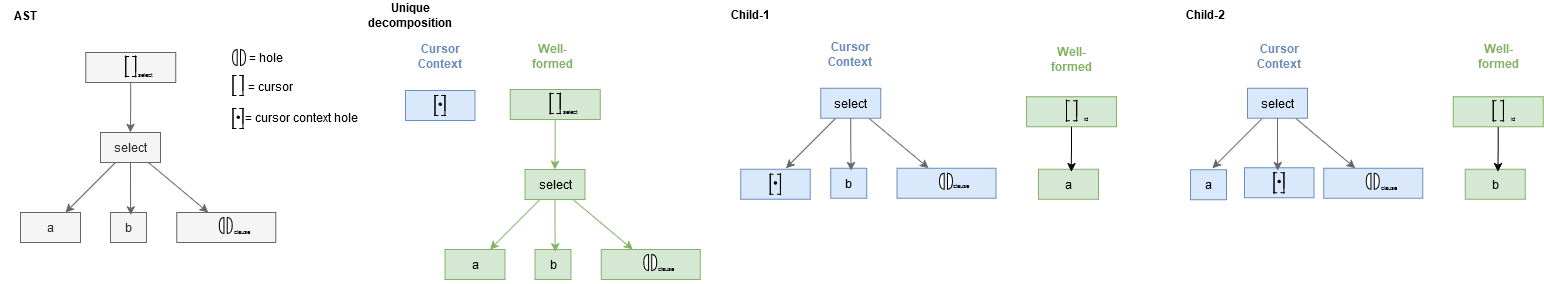
\includegraphics[width=1\textwidth]{img/sql-decomposition-and-movement.drawio.png}
\end{frame}

\begin{frame}[hvid]
    \frametitle{Picking good language examples}
    \begin{itemize}
        \item What makes a good set of examples?
              \begin{itemize}
                  \item Different paradigms and purposes:
                        \begin{itemize}
                            \item General purpose programming language
                            \item Domain-specific language
                            \item Markup language
                        \end{itemize}
                  \item Popular (present in GitHub top 30 ranking\footfullcite{prog-lang-metrics})
              \end{itemize}
              \pause
        \item Examples:
              \begin{itemize}
                  \item C
                  \item SQL
                  \item \LaTeX
              \end{itemize}
    \end{itemize}
\end{frame}

\begin{frame}[fragile]
    \frametitle{Picking good language examples (Continued)}

    \begin{multicols}{2}
        \begin{itemize}
            \item A C program with syntax errors

        \end{itemize}
        \columnbreak
        \begin{lstlisting}[language=c]
int main() {
    int x = 0;
    for (int i; i < 5; i++) {
        x++<@\textcolor{green}{;}@>
    }
    return 0;
}
    \end{lstlisting}
    \end{multicols}
\end{frame}

\begin{frame}[fragile]
    \frametitle{Picking good language examples (Continued)}

    \begin{multicols}{2}
        \begin{itemize}
            \item A SQL query with syntax errors

        \end{itemize}

        \columnbreak

        \begin{lstlisting}[language=sql]
SELECT col-a<@\textcolor{green}{,}@> col-b FROM table
WHERE col-a =<@\textcolor{red}{=}@> 'x';
        \end{lstlisting}
    \end{multicols}
\end{frame}

\begin{frame}[fragile]
    \frametitle{Picking good language examples (Continued)}

    \begin{multicols*}{2}
        \begin{itemize}
            \item A \LaTeX \ document with syntax errors
        \end{itemize}

        \columnbreak

        \begin{lstlisting}[basicstyle=\tiny\ttfamily]
...
\begin{equation}
    \|\vect{v}\| = \sqrt{\sum_{i=1}^n v_i^2<@\textcolor{green}{\}}@>
\end{equation}
...
        \end{lstlisting}
    \end{multicols*}
\end{frame}

\begin{frame}[hvid]
    \frametitle{Generated editor for SQL}
    \includegraphics[width=\textwidth]{img/sql-repl.png}
\end{frame}


\begin{frame}[hvid]
    \frametitle{Conclusions}
    \begin{itemize}
      
    \item We have presented a general editor calculus and shown how to
      encode it in a typed $\lambda$-calculus.
        \item We have an implementation. Some editor expressions
          are yet to be implemented. Currently, we still need to
              \begin{itemize}
                  \item Handle context-sensitive syntax
                  \item Implement views of code being edited
              \end{itemize}
    \end{itemize}
\end{frame}


\begin{frame}[hvid]
    \frametitle{Future work}

    \begin{itemize}
        \item Finish the implementation.
        \item Consider a more concise implementation (maybe in Haskell)
    \end{itemize}
\end{frame}


\end{document}
%%% Local Variables:
%%% mode: latex
%%% TeX-engine: luatex
%%% TeX-master: t
%%% End:
